\section{Methods}

% ------------------------------------------------------------------------------
\begin{frame}{Debiased: good units now look like bad units}
  \centering
  \begin{tikzpicture}[node distance=4mm and 10mm,
      codebox/.style={box, align=left, font=\ttfamily\scriptsize, inner sep=3pt}]
    \node[codebox, draw=WarnDraw, fill=WarnFill] (orig) {%
      \textcolor{OIvermil}{\textbf{static void}} G2B()\ \{ ALLOCA \}\\
      \textcolor{OIvermil}{\textbf{static void}} B2G()\ \{ malloc \dots\ free \}\\
      void good()\ \{ G2B(); B2G(); \}};
    \node[lbl, above=1mm of orig] {Original good unit};
    \node[codebox, draw=DataDraw, fill=DataFill, right=10mm of orig, yshift=7mm] (g2b) {%
      {\sffamily\bfseries G2B:}\ void sym\_0()\ \{ ALLOCA \dots\ \}};
    \node[codebox, draw=DataDraw, fill=DataFill, below=4mm of g2b.south west, anchor=north west] (b2g) {%
      {\sffamily\bfseries B2G:}\ void sym\_0()\ \{ malloc \dots\ free \}};
    \node[lbl] at ($(g2b.north)+(0,3mm)$) {Debiased: one good unit per group};
    \draw[arr] (orig.east) -- (g2b.west);
    \draw[arr] (orig.east) -- (b2g.west);
  \end{tikzpicture}
  \vspace{6pt}
  \begin{itemize}
    \item One entry function; wrapper and \code{static} removed
    \item Good unit is either G2B (no heap) or B2G (malloc + free)
    \item Bad units unchanged; same shape and length
  \end{itemize}
\end{frame}

% ------------------------------------------------------------------------------
\begin{frame}[fragile]{DeadFree adds a \code{free} that never runs}
  \begin{columns}[T]
    \begin{column}{0.48\textwidth}
      \textbf{bad} + dead free $\Rightarrow$ still \alert{leak}
\begin{lstlisting}[style=unit]
static const int sym_7 = 5;
data = (char *)malloc(100);
(*\hlc{if (sym\_7 != 5) \{ free(data); \}}*)
\end{lstlisting}
      \textbf{good}: real free, always-true guard
\begin{lstlisting}[style=unit]
(*\hlc{if (sym\_7 == 5) \{ free(data); \}}*)
\end{lstlisting}
    \end{column}
    \begin{column}{0.48\textwidth}
      \textbf{Placebo} (control): same guard, no free
\begin{lstlisting}[style=unit]
if (sym_7 != 5) { printLine("..."); }
\end{lstlisting}
      \vspace{4pt}
      \begin{itemize}
        \item Labels do not change
        \item Both labels now contain a \code{free}
        \item Only path feasibility decides
      \end{itemize}
    \end{column}
  \end{columns}
  \vfill
  {\scriptsize Dead frees in both labels; G2B goods get one too. All 3,316 units per layer compile (gcc, clang); labels re-checked by running them.\par}
\end{frame}

% ------------------------------------------------------------------------------
% src: fold sizes juliet_full/data/build/layer3.jsonl (set=eval: fold0 15 variants/472 groups, fold1 12/424, fold2 12/432)
\begin{frame}{We test on unseen flow variants}
  \centering
  \begin{tikzpicture}[x=0.071mm, y=1mm]
    % widths proportional to groups: dev 330, fold0 472, fold1 424, fold2 432 (total 1,658)
    \foreach \x/\w/\c/\name/\sub in {0/330/NeutFill/dev/9 variants, 330/472/HeroFill/fold 0/15 variants,
        802/424/HeroFill/fold 1/12 variants, 1226/432/HeroFill/fold 2/12 variants}{
      \fill[\c, draw=NeutDraw, line width=0.5pt] (\x,0) rectangle ++(\w,9);
      \node[font=\small] at (\x+\w/2,5.6) {\textbf{\name}};
      \node[font=\scriptsize, text=NeutDraw] at (\x+\w/2,2.6) {\sub};
    }
    \draw[decorate, decoration={brace, amplitude=4pt, mirror}, NeutDraw] (0,-1) -- (330,-1)
      node[midway, below=4pt, lbl] {frozen: prompts, $\tau$, checkpoints};
    \draw[decorate, decoration={brace, amplitude=4pt, mirror}, HeroDraw] (330,-1) -- (1658,-1)
      node[midway, below=4pt, lbl, text=HeroDraw] {eval: 39 unseen variants, 2,656 units};
  \end{tikzpicture}
  \vspace{8pt}
  \begin{itemize}
    \item Split by Juliet flow variant, not by unit
    \item Fine-tuning: train on two folds, predict the third
    \item Macro-F1 (leak = positive), family-cluster bootstrap CI
    \item Speed: median latency per unit, one request at a time
  \end{itemize}
\end{frame}

% ------------------------------------------------------------------------------
\begin{frame}{L1--L3: ask for the verdict, with more or less help}
  \centering
  \renewcommand{\arraystretch}{1.2}
  \begin{tabular}{@{}lll@{}}
    \toprule
    & Prompt input & Answer \\
    \midrule
    \textbf{L1} direct & unit code & leak / no leak \\
    \textbf{L2} few-shot & + fixed dev examples & leak / no leak \\
    \textbf{L3} analysis-guided & + Clang SA warnings as evidence & leak / no leak \\
    \bottomrule
  \end{tabular}
  \vspace{10pt}
  \begin{columns}[T]
    \begin{column}{0.47\textwidth}
      \textbf{Generative} model\\
      {\small writes the label as JSON\\DeepSeek, Qwen3.5-4B, VulnLLM-R}
    \end{column}
    \begin{column}{0.47\textwidth}
      \textbf{Decision} model\\
      {\small one forward pass, reads P(Yes) vs P(No)\\Jev, Intern-Decision-4B, ours}
    \end{column}
  \end{columns}
  \vfill
  {\scriptsize Same prompt text for every model (VulnLLM-R: its authors' prompt); temperature 0, thinking off; prompts frozen on dev.\par}
\end{frame}

% ------------------------------------------------------------------------------
% src: L4 = juliet_full/llm/l4/leak.dl (v3); L4-D = juliet_full/l4d/README.md (contract), juliet_full/l4d/l4d.dl,
%   question templates juliet_full/l4d/templates.py
\begin{frame}{L4 and L4-D: the model supplies facts, Datalog decides}
  \centering
  \begin{tikzpicture}[node distance=3mm and 5mm]
    % L4
    \node[box] (c1) {unit\\code};
    \node[warn, right=of c1] (llm) {LLM\\{\scriptsize generates}};
    \node[data, right=10mm of llm, font=\scriptsize, align=left] (f1) {\texttt{alloc free assign}\\\texttt{call dead(line)} \dots};
    \node[hero, right=of f1] (dl1) {Souffl\'e\\{\scriptsize \texttt{leak.dl}}};
    \node[box, right=of dl1] (o1) {leak?};
    \node[lbl, left=1mm of c1, font=\small\bfseries, text=Ink] {L4};
    \draw[arr] (c1) -- (llm); \draw[arr] (llm) -- node[lbl, above] {JSON} (f1); \draw[arr] (f1) -- (dl1); \draw[arr] (dl1) -- (o1);
    % L4-D
    \node[box, below=11mm of c1] (c2) {unit\\code};
    \node[box, right=of c2] (sites) {parser\\{\scriptsize sites}};
    \node[data, right=of sites, align=left, font=\scriptsize] (q) {typed yes/no\\questions};
    \node[warn, right=of q] (dm) {decision\\model};
    \node[hero, right=10mm of dm] (dl2) {Datalog\\{\scriptsize rules v1}};
    \node[box, right=of dl2] (o2) {leak?};
    \node[lbl, left=1mm of c2, font=\small\bfseries, text=Ink] {L4-D};
    \draw[arr] (c2) -- (sites); \draw[arr] (sites) -- (q); \draw[arr] (q) -- (dm);
    \draw[arr] (dm) -- node[lbl, above] {$p\geq\tau$} (dl2); \draw[arr] (dl2) -- (o2);
  \end{tikzpicture}
  \vspace{6pt}

  {\small
  \begin{tabular}{@{}ll@{}}
    \code{heap(a)} & Does the call at line $a$ allocate heap memory? \\
    \code{exec\_any(s)} & Can the (masked) statement $s$ run on \emph{at least one} run? \\
    \code{exec\_all(s)} & Does $s$ run on \emph{every} run? \\
    \code{rel(f,a)} & Does the release at $f$ free the block from $a$? \\
    \code{realloc\_safe(r)} & If \code{realloc} at $r$ fails, is the old block still released? \\
  \end{tabular}\par}
\end{frame}

% ------------------------------------------------------------------------------
% src: juliet_full/l4d/l4d.dl (rules v1, verbatim modulo the unit argument)
\begin{frame}[fragile]{Three rules turn the answers into a verdict}
  \begin{columns}[c]
    \begin{column}{0.56\textwidth}
\begin{lstlisting}[style=dl]
freed(a) :- rel(f, a), exec_all(f).
leak(a)  :- heap(a), exec_any(a), !freed(a).
leak(a)  :- realloc(a), exec_any(a),
            !realloc_safe(a).
unit_leak :- leak(_).
\end{lstlisting}
    \end{column}
    \begin{column}{0.42\textwidth}
      \begin{itemize}
        \item A leak: \emph{may} be allocated, \emph{not must} be freed
        \item The dead free fails \code{exec\_all}
        \item The model answers small local questions, not the whole verdict
      \end{itemize}
    \end{column}
  \end{columns}
  \vspace{8pt}
  {\small Facts: \code{heap}, \code{exec\_any}, \code{exec\_all}, \code{rel}, \code{realloc\_safe} from the model;
  site lists (\code{realloc}) from the parser. Run by Souffl\'e; a Python twin agrees on every unit.\par}
\end{frame}

% ------------------------------------------------------------------------------
% src (lectures, verified with pdftotext 2026-11-24 in /home/barton/Documents/projects/cs224/slides/):
%   Lecture 10 "Pointer Analysis": "Allocation-Site Abstraction ... one abstract object per allocation site";
%     analysis scope "Demand-driven: only compute points-to information for the pointers that may affect specific sites of interest".
%   Lecture 3-4 "Data Flow Analysis": "may analysis ... over-approximation; must analysis ... under-approximation";
%     Reaching Definitions (may), Available Expressions (must).
%   Lecture 17 "Datalog-Based Program Analysis": EDB/IDB predicates, negation !B(...), pointer/taint analysis via Datalog.
%   Lecture 1 "Introduction" (sound / complete); Lecture 18 "Soundiness": "Virtually all published whole-program
%     analyses are unsound when applied to real programming languages".
\begin{frame}{The design follows the course's program-analysis ideas}
  \small
  \renewcommand{\arraystretch}{1.15}
  \begin{tabular}{@{}p{0.36\linewidth}p{0.58\linewidth}@{}}
    \toprule
    L4-D element & Course idea (lecture) \\
    \midrule
    one fact set per \code{malloc}/\code{new} site & allocation-site abstraction (L10 Pointer Analysis) \\
    \code{exec\_any} / \code{exec\_all} & may vs must analysis, cf.\ reaching definitions vs available expressions (L3--4 Data Flow Analysis) \\
    \code{leak} = may-allocated $\wedge$ $\neg$must-freed & may/must safe approximation (L3--4) \\
    facts $\to$ rules with negation & Datalog-based program analysis: EDB, IDB, \code{!} (L17) \\
    ask only what \code{leak} needs & demand-driven analysis (L10) \\
    \midrule
    \textcolor{NeutDraw}{model facts can be wrong} & \textcolor{NeutDraw}{no soundness guarantee; real analyzers are ``soundy'' too (L1, L18)} \\
    \bottomrule
  \end{tabular}
\end{frame}

% ------------------------------------------------------------------------------
% src: juliet_full/l4d_ft/prune.py (needed()), juliet_full/l4d_ft/results/scores/prune_test.json
%   (questions_per_unit_eval medians; pred_diffs for gold and stored lora_l4d answers, all folds and layers)
\begin{frame}{Asking only what the rules read halves the questions}
  \centering
  \begin{tikzpicture}[node distance=4mm and 9mm, every node/.style={font=\small}]
    \node[hero] (leak) {\code{leak(a)}};
    \node[data, left=of leak, yshift=8mm] (heap) {\code{heap}\\{\scriptsize alloc sites}};
    \node[data, left=of leak, yshift=-8mm] (any) {\code{exec\_any}\\{\scriptsize alloc, realloc sites}};
    \node[box, right=of leak] (freed) {\code{freed(a)}};
    \node[data, right=of freed, yshift=8mm] (rel) {\code{rel}\\{\scriptsize all pairs}};
    \node[data, right=of freed, yshift=-8mm] (all) {\code{exec\_all}\\{\scriptsize release, realloc sites}};
    \draw[arr] (heap) -- (leak); \draw[arr] (any) -- (leak);
    \draw[arr] (freed) -- node[lbl, above] {!} (leak);
    \draw[arr] (rel) -- (freed); \draw[arr] (all) -- (freed);
  \end{tikzpicture}
  \vspace{6pt}
  \begin{itemize}
    \item Backward from \code{leak}: drop facts no rule reads (e.g.\ \code{exec\_*} on plain statements)
    \item Median questions per DeadFree unit: \res{df-x}{q_full_layer3} $\to$ \alert{\res{df-x}{q_pruned_layer3}}
    \item Verdict differences on all 4 layers: \res{df-x}{prune_diffs_total}
  \end{itemize}
  \vfill
  {\scriptsize Optimized inference, post-hoc (user-approved 2026-11-24); same trained models, same $\tau$. ``L4-D (opt.)'' below.\par}
\end{frame}

% ------------------------------------------------------------------------------
% src: oracle and attribution = juliet_full/analysis/l4d_peek/fact_error_attribution.out.txt (gold facts substituted per
%   fact type, rules frozen, eval 2,656 units); oracle FP all variant-12 goods: juliet_full/l4d/REPORT_stage1.md
\begin{frame}{With correct facts the rules are near-perfect; \code{exec\_all} is the bottleneck}
  \begin{columns}[c]
    \begin{column}{0.58\textwidth}
      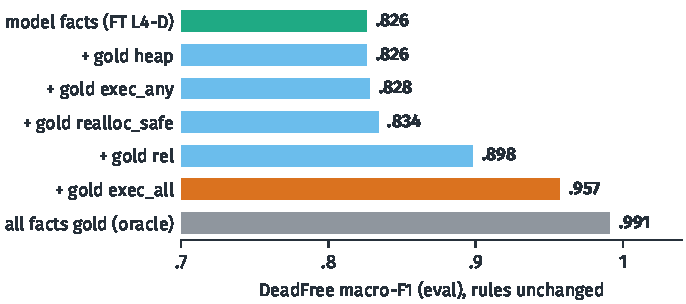
\includegraphics[width=\linewidth]{figures/df_attribution.pdf}
    \end{column}
    \begin{column}{0.40\textwidth}
      \begin{itemize}
        \item All gold facts: \res{df-x}{attr_layer3_all}, FN \res{df-x}{attr_layer3_all_fn}, FP \res{df-x}{attr_layer3_all_fp}
        \item Gold \code{exec\_all} only: \res{df-x}{attr_layer3_none} $\to$ \alert{\res{df-x}{attr_layer3_exec_all}}
        \item Errors come from wrong facts, mostly path feasibility
      \end{itemize}
    \end{column}
  \end{columns}
  \vfill
  {\scriptsize Gold facts from dynamic analysis. Oracle FPs: random-branch goods (flow variant 12) the path-insensitive rules cannot see.\par}
\end{frame}

% ------------------------------------------------------------------------------
% src: juliet_full/l4d/README.md (training contract), juliet_full/l4d_ft/PROGRESS.md (~68 min/fold, 2x RTX 3090 DDP),
%   decision_ft lane report (LoRA r16, 32.5 M trainable = 0.70 %)
\begin{frame}{Fine-tuning: one recipe, different labels per strategy}
  \centering
  \begin{tikzpicture}[node distance=4mm and 12mm]
    \node[box, align=center] (in) {prompt\\{\scriptsize L1 / L3 / L4-D question}};
    \node[hero, right=of in, align=center] (m) {Qwen3.5-4B\\+ LoRA};
    \node[data, right=of m, align=center] (s) {$s=\ell_{\text{Yes}}-\ell_{\text{No}}$};
    \draw[arr] (in) -- (m); \draw[arr] (m) -- node[lbl, above] {1 pass} (s);
  \end{tikzpicture}
  \vspace{2pt}

  \small
  \renewcommand{\arraystretch}{1.1}
  \begin{tabular}{@{}lll@{}}
    \toprule
    Strategy & Training label & Loss \\
    \midrule
    L1, L3 & unit label (leak / no leak) & balanced CE + bad\,$>$\,good ranking \\
    L4-D & fact label from \textbf{dynamic analysis} & CE balanced per (question type, label) \\
    \bottomrule
  \end{tabular}
  \vspace{4pt}
  \begin{itemize}\small
    \item LoRA r16, $\alpha$32 on all LM linear layers: 32.5\,M weights (0.70\,\%); head from tied Yes/No rows
    \item Fact labels: gcov coverage, alloc/free trace, \code{realloc} failure injection; rules frozen
    \item 3-fold CV by flow variant; dev picks checkpoint and $\tau$; $\approx$68\,min/fold on 2$\times$ RTX 3090; L2 not trained
  \end{itemize}
\end{frame}
